%!TEX root = ../thesis.tex
%*******************************************************************************
%*********************************** First Chapter *****************************
%*******************************************************************************

\chapter{Introduction}  %Title of the First Chapter

\ifpdf
     \graphicspath{{Figs/Chapter1/}}
\else
    \graphicspath{{Chapter1/Figs/Vector/}{Chapter1/Figs/}}
\fi


%********************************** %First Section  **************************************

\section{Overview} %Section - 1.1 

\emph{"... as they say, your model is only as good as the data you have. \newline So it all starts with the data ..."} \newline
\indent \indent - Nyalleng Moorosi, \emph{Deep Learning Indaba} (2017). \newline 

Artificial intelligence (AI) is the imitation of human-level intelligence by machines. Human beings are capable of extracting information from a passage of text and transforming that information into a mental model of objects and relationships between those objects. As stated by Nyalleng Moorosi, the model is only as good as the data you give it, this is true for both human mental models as well as machine constructed models. \newline 
Human models are often confined to a finite domain ~\citep{staab2010handbook}, for example a mental model might be one of the entertainment industry. The entertainment industry contains objects such as films, actors and actresses, characters and awards. These objects have relationships between them, such as "stared in", "worked along side", "a character in", and "was nominated for". Humans can use this model to easily reason about new relationships between the objects that weren't mentioned in passage of text. For example the text may say that Chadwick Boseman stared in a movie called Black Panther, and using that information we can reason that Chadwick Boseman "is an" actor. \newline
We use these models to read and understand other passages of text, in conversations with other people, and to help us answer questions. The set of objects and the relationships between them, within a domain, can be thought of as knowledge. Figure 1.1. shows what knowledge about the entertainment industry might look like. \newline

\begin{figure}
  	\caption{Objects and the Relationships between Them}
   	\centering
    	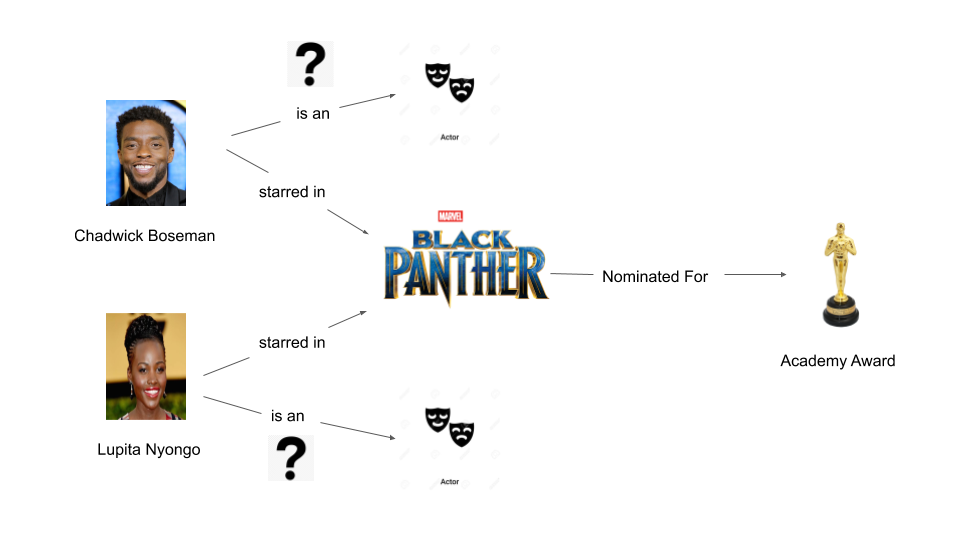
\includegraphics[width=\textwidth]{Objects_and_the_Relationships_Between_Them}
\end{figure}

\textbf{Challenges}. Reasoning about knowledge expressed in natural language ~\citep{minervini2019differentiable} is simple for humans, but trying to imitate this behaviour in computers reveals its underlying complexity. \newline 
The first task is providing a mechanism for perceiving syntax. Humans recognise text as sequences of words, and words as a sequence of characters. Characters can belong to different writing systems which can be dense - have a few characters used in a large number of combinations, or sparse - have a very large number of characters used in less combinations ~\citep{Hua2010}. A computer has to first be able to perceive these characters. \newline
The second task is even more challenging: semantics. Semantics is the meaning of words in language ~\citep{chomsky1955logical}. Semantics is what allows humans to understand each other in conversation, through written text, and through visual imagery. Semantics allow us to understand that an actor is a thing, and that things can have relationships with other things. Giving computers the capability to semantic understanding is very challenging because of the "messiness" of language. If a person is shown a word in the singular, and a word in the plural, for example "film" and "films" a person will most likely understand that there is not much difference in meaning between the two words, a computer may interpret them as having completely different meanings. Different words can also have similar meanings, for example "movie" and "film". Capturing this statistical similarity once again challenging for machines. And finally the order in which words are seen provides context, for example, the word "star" has completely different meaning in "Chadwick Boseman is a movie star" and "Black Panther looked up into the night sky an saw a star". \newline
The third task is organising information in such a way as to be able to reason about the knowledge it conveys. Humans build mental models using default reasoning ~\citep{reiter1980logic} - believing that most Objects A have relationship Relationship with Object B, with a small number of exceptions. For example we could believe that films (Object A) have not won (Relationship) an Oscar (Object B), except for films such as Black Panther (Object B). We will believe this is true for any given movie, unless we are familiar enough with movie history to identify the exceptions. Formallly, the default beliefs we hold are facts, and this process of reasoning allows us to infer new facts - plausible relationships between objects. \newline
In order to allow computers to use the same method of reasoning, data has to be structured as facts and stored in a database. Such a database is called a knowledge base (KB) ~\citep{carlson2010toward, angeli2013philosophers}  and is modelled on ontologies. A KB is used to store facts, which encode knowledge about a domain. These facts are modelled as triples - subject, predicate, object, where the subject and object are entities, and the predicate is the relation between the two entities. For example, a fact (triple) in the entertainment KB would be Black Panther (subject/entity) is a (predicate/relation) super hero (object/entity). This model is derived from the resource description framework model of the semantic web ~\citep{bizer2009dbpedia}. \newline
The problem with this approach is facts are either present in the database or they are not i.e. questions can be answered exactly, or they cannot. There is no measure of plausibility that can be used to accept new potential facts, or discard implausible facts ~\citep{koller2007introduction}. \newline
\textbf{Encourging Progress}. The task of reasoning about knowledge expressed in natural language is a daunting one, however we have seen tremendous progress in statistical relational learning. The first major progress was the integration of the bilinear tensor product and neural networks ~\citep{socher2013reasoning}. This approach effectively extended linear tensor factorisation techniques to nonlinear tensor factorisation. The approach simultaneously introduced using pre-trained word embeddings to initialise entities and relations, instead of using randomly initialised word vectors. In this one approach, both reasoning and semantic representations were extended. \newline
The second time major progress was realised was with the use of complex valued embeddings for link prediction ~\citep{trouillon2016complex}. This approach extended the Bilinear Tensor product by making use of Hermitian dot product, the complex counterpart of the standard dot product between real vectors. The approach proposes complex vectors can effectively capture antisymmetric relations while retaining the efficiency benefits of the dot product. This was achieved by using representations with complex embeddings $\mathbb{C}$, allowing the model to capture the semantic meaning depending on the order of the embeddings. \newline 
The previous two milestones relied on shallow models that could scale to large datasets. Up until that point, research in link prediction had focused on minimising the parameterisation of models. Convolutional networks are parameter efficient models, and major progress was again realised with the use of convolutional deep learning models for link prediction ~\citep{dettmers2018convolutional}. The approach makes use of 2D embedding representations which allow the modelling of a high number of interactions between embeddings. \newline 
Despite this progress, we've yet to see this method knowledge-based reasoning deployed to real-life applications. Alternative methods such as approaches to solving the Stanford Question Answering Dataset (SQuAD) ~\citep{rajpurkar2016squad}, General Language Understanding Evaluation (GLUE) benchmarks ~\citep{liu2019roberta}, and the Alexa Prize ~\citep{ram2018conversational}, have seen greater commercial adoption. Applications of link prediction seem to be more focused on the evolution of relational databases, and have so far found utility in laboratory information management systems ~\citep{HARROW20192068}. \newline
\textbf{Remaining Challenges}. Perhaps the lack of adoption in link prediction is due to the current neural factorisation model state-of-the-art (SOTA) performance in open-domain question answering: 25.20\% ~\citep{balazevic2019hypernetwork}. A possible explanation for why SOTA performance is so low is that Toutanova and Chen ~\citep{toutanova2015observed} realised inverse relation test set leakage from the training set of FB15k. Because of this test set leakage, simple rule-based models were able to exploit inverse relations in the test set and achieve SOTA performance. Similarly, current neural factorisation model SOTA performance on the less challenging WN18RR dataset is 43.60\%. Dettmers et al. ~\citep{dettmers2018convolutional} created this dataset after discovering a similar test leakage problem in WN18. We can conclude that link prediction SOTA performance has to dramatically improve before wide-spread adoption can be realised. \newline
\textbf{Outline of contributions}. SOTA neural factorisation models ~\citep{balazevic2019hypernetwork, dettmers2018convolutional} introduce relational covariate shift ~\citep{ioffe2015batch}. The models extend the bilinear model ~\citep{jenatton2012latent} by computing subject-predicate transformations using a convolutional operation ~\citep{zeiler2014visualizing}, instead of a dot product. This extension exacerbates covariate shift between the subject and predicate features. We correct for this exacerbated covariate shift by regularising relational filters using batch normalisation. \newline 
Leveraging semantic information ~\citep{NIPS2013_5028} from pre-trained word embeddings ~\citep{mikolov2013distributed} can provide richer representations which can be used for improved inference during reasoning. At the same time, link prediction benchmark datasets often only present one or two occurrences of facts, leading to limited opportunity in capturing the appropriate representation distributions for entities and relations. We integrate pre-trained word embeddings into SOTA neural factorisation model training to compensate for this sparsity in representational data, providing richer context with which to perform reasoning. \newline
\textbf{Long-term Motivations}. Reasoning about knowledge expressed in natural language is one of the strongest measures of intelligence possessed by humans. This capability allows the discourse, debate and dialogue. In order for humans to realise artificial general intelligence (AGI), this skill has to be mastered by machines. Potential applications that can be designed using such technology have profound implications for all aspects of society including in education - such as tutoring systems, health - primary health frontline assistants, and science - from applications such as astronomy to energy research. Practical implementations of AGI will be grounded in natural language and the internet. This works aims to contribute implementations that help in methodology understanding toward the realisation of full AGI.  \newline
\textbf{Short-term Motivations}. We note the poor performance in open domain question answering currently achieved by SOTA neural factorisation models ~\citep{balazevic2019hypernetwork, dettmers2018convolutional}. A sensible implementation of AGI would use heterogeneous information sources from the internet ~\citep{angeli2013philosophers}. Extracting information from the web, constructing or expanding knowledge bases, and then answering questions ~\citep{shalaby2019beyond} is currently the most successful paradigm for open domain question answering. Given the most successful models using this paradigm have poor performance, there is an opportunity to refine existing techniques in the aim to make them more useful in answering questions in this way. Revolutionising existing methods that try to solve AI tasks by making use of deep learning techniques has seen tremendous progress in fields such as computer vision ~\citep{hudson2018compositional}  and natural language processing ~\citep{peters2018deep}. Neural factorisation approaches should attempt further integration of deep learning methods, with the adoption of practices from such fields applied to training, reasoning and knowledge representation. Given that deep learning itself is modelled after human after the human mind, it seems sensible to try to bring SRL into closer alignment with methods of reasoning used by humans. \newline
\textbf{Challenges of this approach.}  In order to answer open-domain questions, the domain in which the knowledge belongs needs to be defined. Facts about that domain then need to be populated. Typically this is achieved by scanning documents written in natural language on the internet ~\citep{fader2011identifying, dong2014knowledge} and populating a knowledge base. Given the heterogeneity of these data sources, it can be difficult consolidating the information into a central datastore which can the be used to perform inference.  Related to the problem of centralising knowledge, the number of facts within a domain can range from hundreds of thousands, to millions. The poses a sample scarcity or model density problem. In the former, it becomes a challenge to adequately model the probability distributions of plausible relations given the in frequency in observations of facts about a particular subject. In the latter, the required large parameterisation of  models is needed to encode knowledge within the domain. \newline
An additional challenge to this method of question answering are the compute resources required to perform inference. For any given question, current methods perform an inference test on every entity within the knowledge base. This is not a challenge knowledge bases with a small number of entities, for example tens of thousands of entities, however this poses a serious scalability problem from knowledge bases with entities in the millions. This compute problem presents significant opportunity for more scalable inference implementations. Similarly, question answering is modelled as a classification task, where the classification categories are the entities themselves. This means small numbers of target categories are in the tens of thousands, and can be as large as millions of categories. This seems like an impractical method of modelling question answering and also presents significant opportunity for improvement. 


%********************************** %Second Section  *************************************

\section{Related Work} %Section - 1.2 

\textbf{Reasoning about Facts.} This dissertation aims to extend research that aspires to give computers the capability of human-like reasoning ~\citep{bordes2011learning} in open domain question answering ~\citep{hakimov2019evaluating}. Early work in this area focused on learning deterministic logical concepts based on symbolic frameworks ~\citep{hohenecker2017deep} which were used for formal reasoning. Later, attempts to relax formal reasoning and make use of more flexible embedding representations of natural language inspired research in statistical relational learning (SRL) ~\citep{koller2007introduction}. Link prediction is an SRL approach to human-like reasoning that makes use of knowledge bases ~\citep{balazevic2019hypernetwork, dettmers2018convolutional, socher2013reasoning}. \newline
Early approaches to reasoning over facts in KBs were attempted using tensor factorisation ~\citep{nickel2011three} to model entity-relational interactions. Nickel et al. (2011) implemented RESCAL, a model that uses the bilinear tensor product to model interactions where entities are expressed as vectors and and the relation between them is represented as a full rank matrix ~\citep{nickel2012factorizing}. The triple is then scored by computing product of pairwise interactions between latent features of the respective representations ~\citep{nickel2015review} and producing a measure of confidence in the fact. RESCAL uses the values of the relational matrix to model block structure patterns, homophily patterns, and anti-correlations. \newline
Translations in the embedding (TransE) of entities by Bordes et al. (2013) ~\citep{bordes2013translating} was another approach tried to model entity-relational interactions. The motivation for this approach was that a lot of KB facts are presented in hierarchies, therefore a translation of the subject by the predication should produce an embedding close to the object. The model translation is thus the natural transformation of the entity and be used to model hierarchical, along with embedding equivalence with the null transformation. \newline
Yang et al. (2015) propose DistMult ~\citep{yang2014embedding}, a bilinear diagonal model which first transforms the subject and object entities into low dimensional vector representations, and then applies a bilinear tensor product operation using a relation matrix with only diagonal elements. This model effectively models a subset of the entity-relational interactions of RESCAL and relies on the entity transformations to generate sufficient semantic representations. The model's bilinear formulation is extremely parameter efficient, but lacking in expressiveness. \newline
ComplEx ~\citep{trouillon2016complex} by Trouillon et al. (2016) is the extension of DistMult into the complex domain. Entities are represented using complex vectors, and relations are represented using a diagonal matrix with complex entries. Complex valued embeddings extend the entity-relational interactions modelling to include antisymmetric interactions. \newline
All these approaches rely on linear composite triple representations. Linear composite triple representations scale well with large datasets but are limited in their expressiveness. In the following we will discuss nonlinear composite triple representations. \newline
Neural Tensor Networks (NTN) were proposed by Socher and Chen et al. (2013) ~\citep{NIPS2013_5028}. NTNs approach link prediction by extending the bilinear tensor product in two ways, 1) They model interactions between subject and object entities using recursive neural network (RSNN). ~\citep{socher2012semantic}. This model constructs a representation that is added to the bilinear tensor product, and then 2) resultant representation is then passed through a neural network. The NTN thus expresses richer semantic information by using the RSNN and increases entity-relational interaction expressiveness using a neural triple representation composition. Socher and Chen also examine the use of pre-trained word embeddings on link prediction. They find models trained using word embeddings outperform models trained using random initialisation. \newline
Hohenecker and Lukasiewicz (2017) extend NTNs by pre-computing object representations as aggregations of all the triples in which which the object plays a part ~\citep{hohenecker2017deep}. They introduce the new mode as a Relational NTN (RTN). Dong et al. (2014) introduce ER-MLP ~\citep{dong2014knowledge, nickel2015review}, a simplification of NTN. This model extends entity-relational interaction model by passing the bilinear tensor product through neural network. ER-MLP also makes use of low dimensional vectors for word embedding representations. \newline 
HolE, by Nicel et al. (2016), uses a  circular correlation to create compositional representations ~\citep{nickel2016holographic}. HolE relies on concatenation of the subject and object entities, directly modelling the relational score on shared semantic features of the entities. The relational vector is then used to project the representation, before a sigmoidal non-linearity is used to complete the composition and score the relation. This approach is particularly adept at modelling anti-symmetric interactions. HolE introduces the concept of dynamically training embeddings to represent observed relations instead of storing static entity and relation embeddings. \newline
Dettmers et al. (2018) introduce ConvE ~\citep{dettmers2018convolutional}. ConvE provides a more expressive model by taking the convolution of triple entities with a 2-dimensional convolutional relational model. The subject vector and the relation vector are each reshaped into a matrix and lengthwise contactinated. A convolution operation is then performed on the matrices where the relation matrix performs the task of the relational filter. The obtained feature maps are then flattened and put through a fully connected layer. Finally, the inner product of the generated representation is taken with all object entity vectors to generate a score for each triple. ConvE  increases the expressiveness by modelling entity-relational interactions  around the entire concatenation line, therefore modelling additional points of interaction between embeddings. \newline
The above modelling approaches form part of latent feature modelling in link prediction. Two other research categories, namely graph modelling and inductive probabilistic logic programming, represent attempts at link prediction. We refer the reader to ~\citep{nickel2015review} for a recent review of approaches. \newline
\textbf{Entity and Relation Representations.} Previous work represented entities and relations using randomly initialised, static vector representations. This approach does not allow the sharing of statistical strength between the words describing each entity ~\citep{socher2013reasoning}. Socher and Chen showed that using pre-trained word embeddings instead of randomly initialised word embeddings improves link prediction model performance. This performance gain can be explained by the cooccurrence statistics used to train word embeddings. The semantic and syntactic similarity between words captured by word embeddings helps identify plausible interactions between entities. For example we would expect film and character entities are collocated in pre-trained embeddings spaces. The following describes approaches used to generate such embeddings. \newline
Word2Vec, introduced by (Mikolov et al. 2013) is an algorithm for training distributed representations of words ~\citep{mikolov2013distributed}. The Skip-Gram model ~\citep{mikolov2013efficient} is one of the modes used by Word2Vec to generate word vectors from very large text vocabularies, in the order of 1.6 billion words. The model essentially attempts to take a centre word, and then tries to predict the probability of seeing a context word either to the right of the centre word, or to the left of the centre word. This context window can be any arbitrary size, for example in the previous example the window size is 1. The Skip-Gram model uses the hierarchical softmax ~\citep{morin2005hierarchical} loss function for classification, a computationally efficient approximation of the full softmax, and employs the subsampling of frequent stop words such as “in”, “the”, and “a”. The continuous bag of words (CBOW) ~\citep{mikolov2013efficient} is an alternative approach to the Skip-Gram model. Here the model tries to predict a target word, given a sequence of context words. The CBOW has the advantage of being faster to train and better representations for more frequent words. \newline
GloVe, by (Pennington et al. 2014) is another unsupervised learning algorithm for generating word embeddings ~\citep{pennington2014glove}. The GloVe model generates word embeddings using the co-occurrence statistics of words in a text vocabulary. The vocabulary is viewed as a global statistics space, and the model begins with a pass over the entire corpus and generates a co-occurrence matrix of a words against all other words in the corpus. GloVe thus captures both global and local statistics of a corpus, a shortcoming of Word2Vec which only captures local corpus statistics. GloVe then attempts to model the co-occurrence statistics between words using a neural network that takes two words as input and scores the co-occurrence statistic as output. The training algorithm then minimises a logarithmic squared error loss that incorporates both global and local corpus statistics. The distributional representation of word embeddings modelling approach that GloVe employs, allows it to outperform Word2Vec on word analogy, word similarity, and named entity recognition tasks. It is thus the chosen word embedding method used in this dissertation.


%********************************** % Third Section  *************************************

\section{Contributions and Outline} %Section - 1.3

In this dissertation we develop models for reasoning about knowledge expressed in natural language applied to open domain question answering. In particular, we develop compensate for covariate shift introduced in convolutional relational filter modelling. We also incorporate the statistical properties of pre-trained word embeddings into neural composition triple representation models for link prediction. \newline
In \textbf{Chapter 2} we discuss training algorithm approaches based on the supervised learning paradigm. We then discuss deep learning models, specifically in relation to convolutional and recurrent neural network models. We provide the mathematical background describing the models, the primary problems they aim to address, as well as examples of applications. We also discuss reguliarsiation techniques used to address the bias/variance trade off. To this end we explore the dropout ~\citep{srivastava2014dropout} and batch normalisation ~\citep{ioffe2015batch} regularisation techniques.   \newline
In \textbf{Chapter 3} we begin by building on top of the NTN model introduce by (Socher and Chen at al. 2013) ~\citep{NIPS2013_5028} and reimplemented in Tensorflow by (Doss et al. 2015) ~\citep{Doss2015}. We begin by analysing the neural compositional strengths of the model, as well as RCNN ~\citep{socher2012semantic} entity augmentations.  We align the training algorithm with modern deep learning techniques including use of the ReLU nonlinearity function ~\citep{xu2015empirical}, dropout integration and early stopping ~\citep{prechelt1998early}. We then build on top of the SOTA model in link prediction using a latent feature modelling approach - HypER - introduced by (Bala\v{z}evi\'c et al. 2018) ~\citep{balazevic2019hypernetwork}. We explore the strengths of neural compositional modelling using the hypernetwork architecture ~\citep{ha2016hypernetworks}. We demonstrate the covariate shift introduced by modelling relational filters using the Hypernetwork architecture, and propose a solution to address this problem, and implement a new model HypER+ with these considerations. We then extend HypER+ to make use of pre-trained word embeddings, taking advantage of semantic statistics modelled using GloVe pre-trained word vectors. \newline
In \textbf{Chapter 4} we introduce the Wordnet ~\citep{miller1995wordnet} and Freebase ~\citep{bollacker2008freebase} link prediction benchmark datasets. We establish baseline accuracy performance metrics using the original NTN Tensorflow model. We then train our proposed new model, and compare our hypothesis against the baseline. We then introduce the WN18 ~\citep{bordes2014semantic} and FB15k ~\citep{bordes2013translating} link prediction benchmarrk datasets, and link prediction benchmark metrics. We implement HypER+ and compare our hypothesis model against the baseline. Finally we introduce the WN18RR ~\citep{dettmers2018convolutional} and FB15k-237 ~\citep{toutanova2015observed} link prediction benchmark datasets. We extend HypER+ to take advantage of GloVe pre-trained embeddings and compare our results against the established baseline metrics using the original HypER model. \newline
Finally, in \textbf{Chapter 5} we summarise the dissertation and examine problems preventing link prediction from use in a greater number of commercial applications. We suggest potential solutions to remaining challenges, and propose future areas of research.


